

Here will see view by view the operation of this software.

\subsection*{Views by Views}

\subsubsection*{Main}
When you open the software, you arrive on the page containing all the \textbf{models}.

\begin{figure}[H]
  \centering

  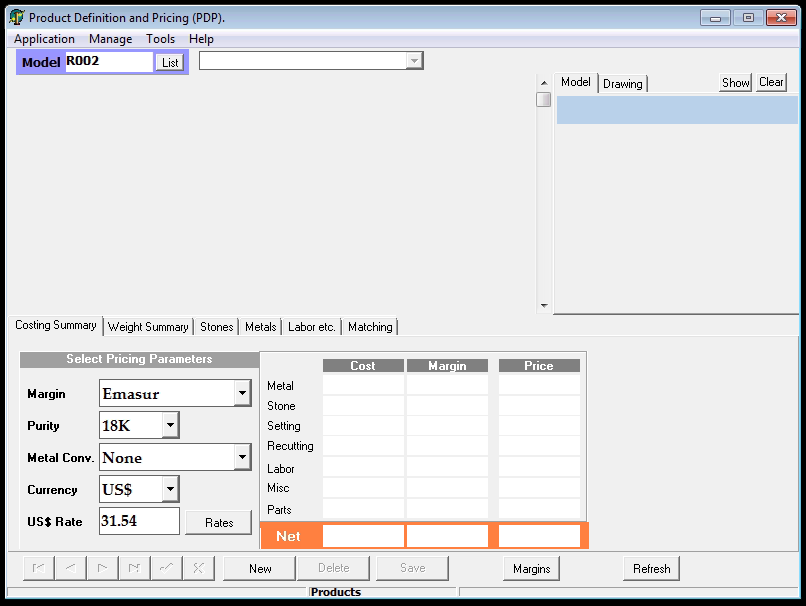
\includegraphics[width=0.4\textwidth]{./images/pdp_default.png}
  \caption{Model list}
\end{figure}

\subsubsection*{Costing Summary}
By default you are on the \texttt{Costing Summary} menu at the lower part of the page.

\begin{figure}[H]
  \centering

  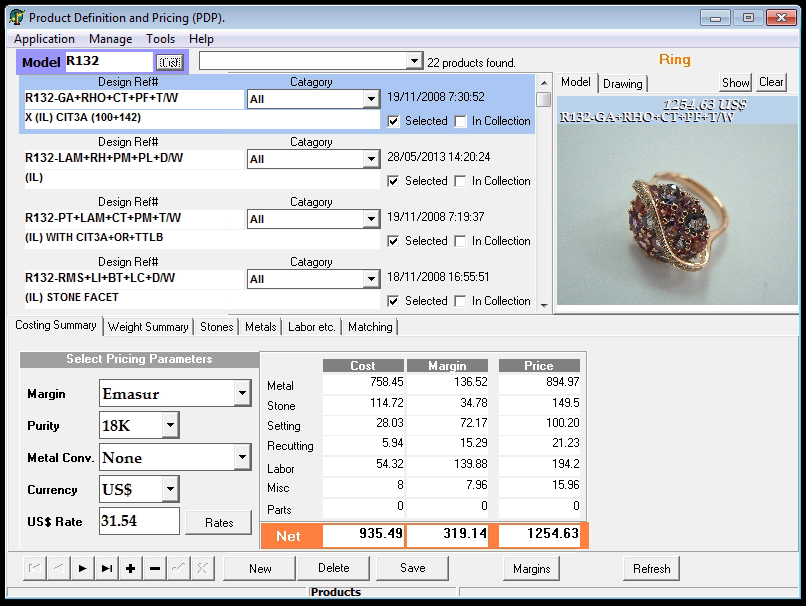
\includegraphics[width=0.4\textwidth]{./images/pdp_model_costingsummary.png}
  \caption{Costing Summary}
\end{figure}

This is one of the most important tables in \texttt{PDP} because it shows the pricing computed by the software. It calculates based on:
\begin{itemize}[leftmargin=*]
  \item \texttt{Margin} depending on the client
  \item \texttt{Purity} of the gold used
  \item \texttt{Metal Conv.}: conversion from the reference metal (White Gold 18K) to the chosen metal
  \item \texttt{Currency} of the cost
  \item \texttt{US\$ Rate}, with the \texttt{Rates} button opening the \texttt{Currencies} page
\end{itemize}
Then you get three columns of pricing details:
\begin{itemize}[leftmargin=*]
  \item \texttt{Cost}: what Rubicon pays
  \item \texttt{Margin}: Rubicon’s margin
  \item \texttt{Price}: the sum, i.e.\ what the client pays
\end{itemize}

\subsubsection*{Model Image}
By default you have an \textbf{image} of the model on the upper right, or by clicking on \texttt{Model}.

\begin{figure}[H]
  \centering

  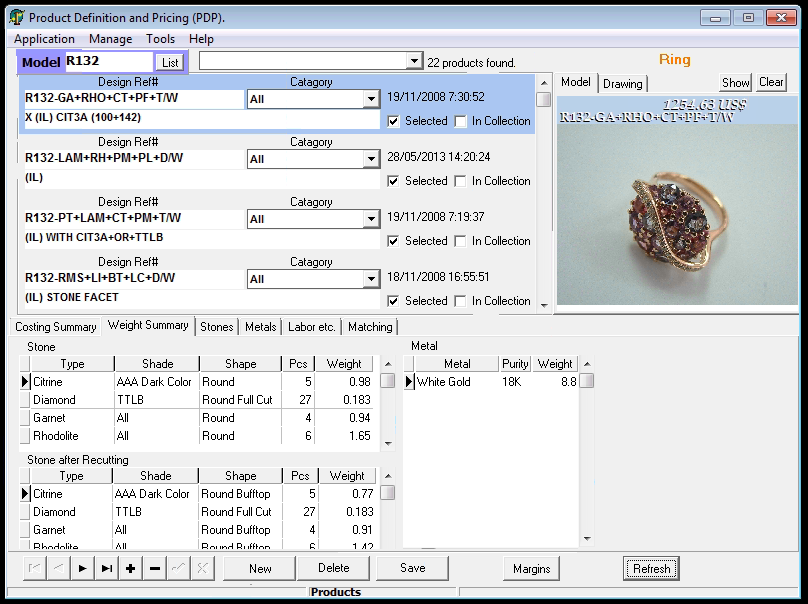
\includegraphics[width=0.4\textwidth]{./images/pdp_model_weightsummary.png}
  \caption{Model Image / Weight Summary}
\end{figure}

\subsubsection*{Drawing}
By clicking on \texttt{Drawing} on the upper right, you can get its identification code.

\begin{figure}[H]
  \centering

  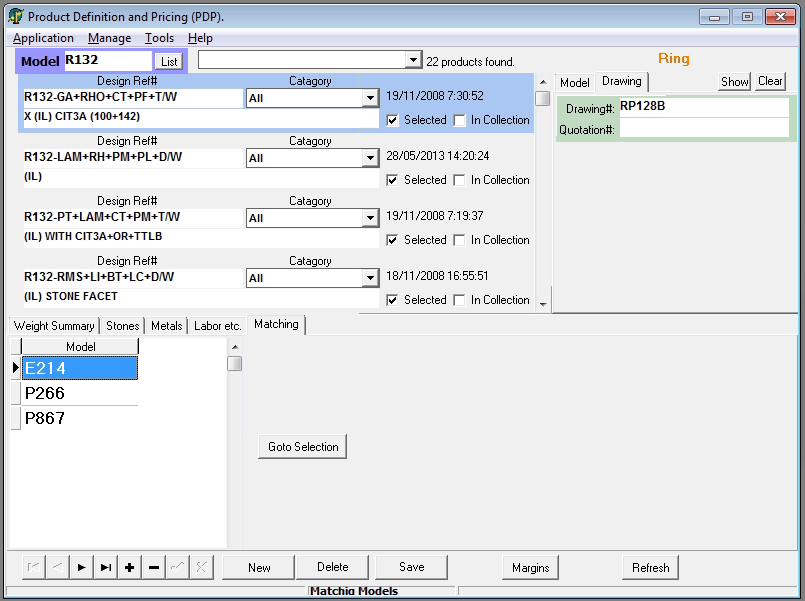
\includegraphics[width=0.4\textwidth]{./images/pdp_model_drawing.png}
  \caption{Drawing Reference}
\end{figure}

\subsubsection*{Model List}
By clicking on \texttt{List} next to \texttt{Model XXXX}, you list all existing models.

\begin{figure}[H]
  \centering

  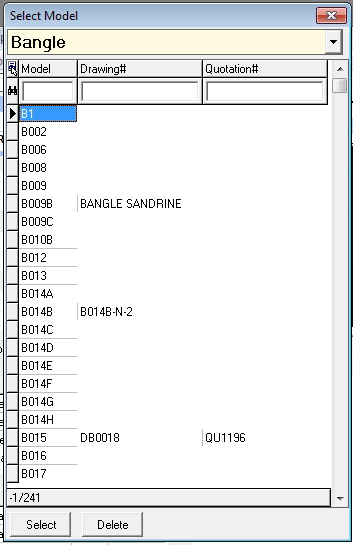
\includegraphics[width=0.4\textwidth]{./images/pdp_selectmodel.png}
  \caption{Select Model List}
\end{figure}

\subsubsection*{New Button}
By clicking on \texttt{New} at the bottom menu, you open the \texttt{Make New Product} view.

\begin{figure}[H]
  \centering

  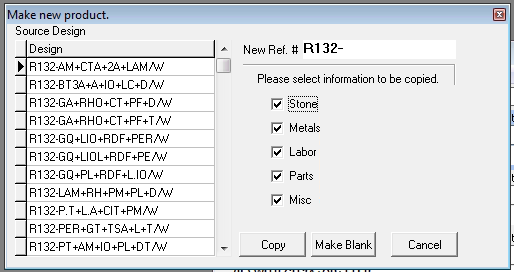
\includegraphics[width=0.4\textwidth]{./images/pdp_makenewproduct.png}
  \caption{Make New Product}
\end{figure}

Here you can:
\begin{itemize}[leftmargin=*]
  \item Create a blank product (\texttt{Make Blank})
  \item Copy an existing product (\texttt{Copy})
\end{itemize}

\subsubsection*{Model Fields}
\paragraph{Product References}
\begin{figure}[H]
  \centering

  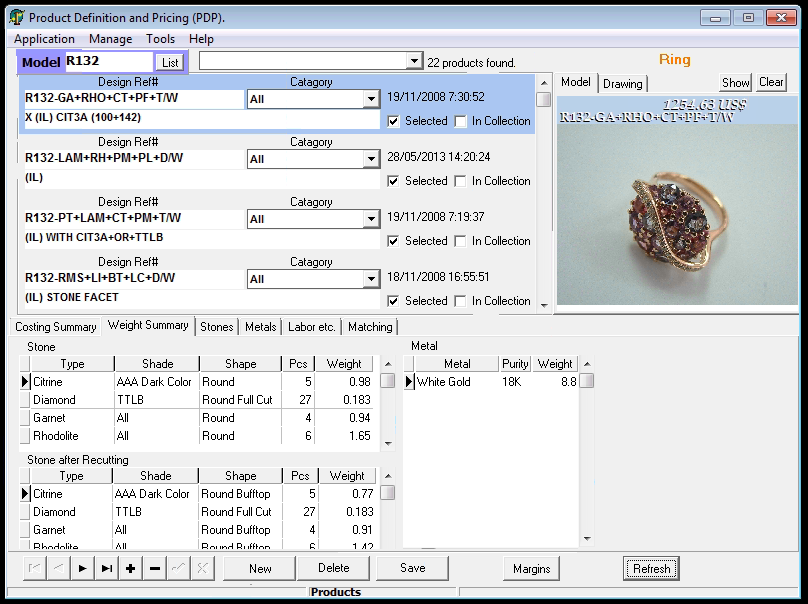
\includegraphics[width=0.4\textwidth]{./images/pdp_model_weightsummary.png}
  \caption{Product References}
\end{figure}

Examples of design references:
\begin{verbatim}
R132-GA+RHO+CT+PF+T/W
R132-PT+LAM+PM+PL+D/W
\end{verbatim}
Format: \texttt{AAXXXB-CS+S1+\dots+SN/W} where
\begin{itemize}[leftmargin=*]
  \item \texttt{AAXXXB}: model type and ID (e.g.\ R for Ring, BA for Bracelet)
  \item \texttt{CS+S1+\dots+SN/W}: center stone, additional stones, and reference metal (W = White Gold 18K)
\end{itemize}

\paragraph{Weight Summary}
\begin{figure}[H]
  \centering

  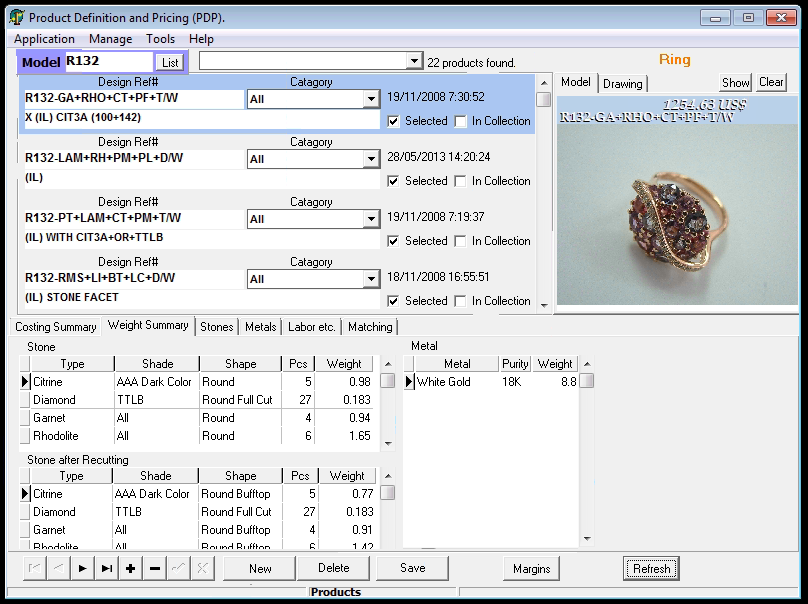
\includegraphics[width=0.4\textwidth]{./images/pdp_model_weightsummary.png}
  \caption{Weight Summary}
\end{figure}
Tables show:
\begin{itemize}[leftmargin=*]
  \item \textbf{Stone}: weights before and after recutting
  \item \textbf{Metal}: weight in chosen metal
\end{itemize}

\paragraph{Stones}
\begin{figure}[H]
  \centering

  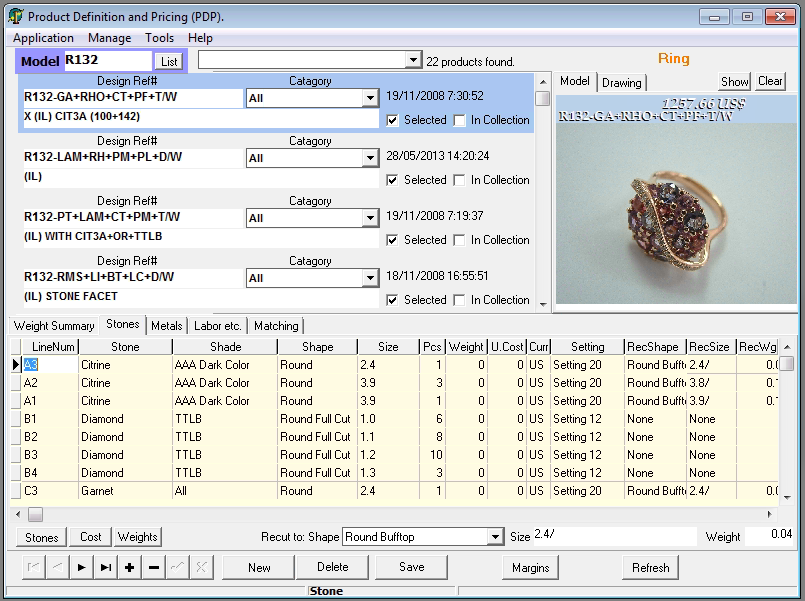
\includegraphics[width=0.4\textwidth]{./images/pdp_model_stones.png}
  \caption{Stones List}
\end{figure}
Fields:
\begin{itemize}[leftmargin=*]
  \item \texttt{LineNum}: unique line key
  \item \texttt{Setting}: labor cost of setting
  \item \texttt{RecShape}, \texttt{RecSize}, \texttt{RecWgt}: recutting parameters and cost
\end{itemize}

\paragraph{Metals}
\begin{figure}[H]
  \centering

  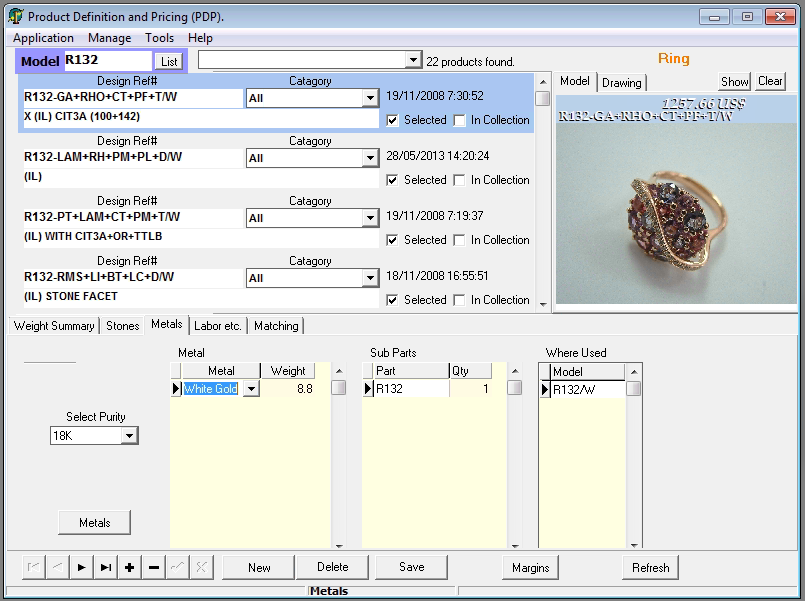
\includegraphics[width=0.4\textwidth]{./images/pdp_model_metals.png}
  \caption{Metals List}
\end{figure}
Add/remove metals with \texttt{+} / \texttt{-}. Clicking on a row opens \texttt{Metal Info}.

\paragraph{Labor etc.}
\begin{figure}[H]
  \centering

  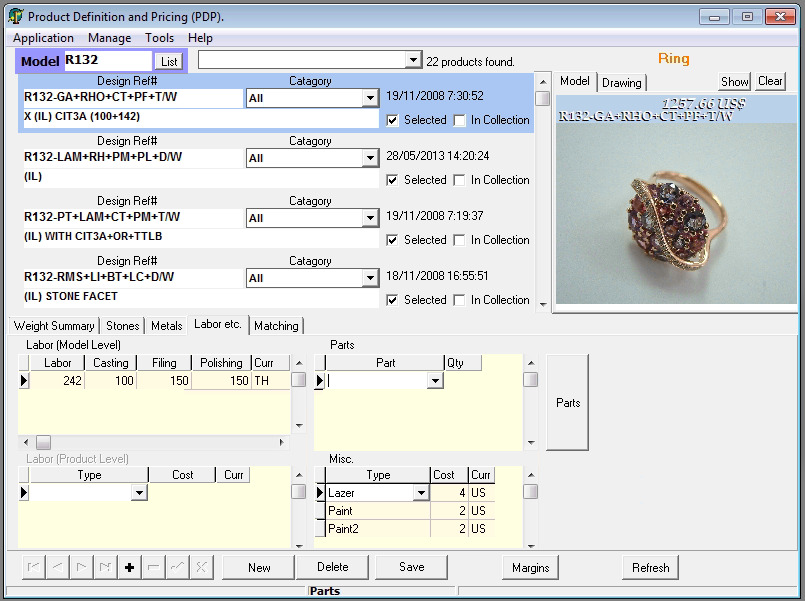
\includegraphics[width=0.4\textwidth]{./images/pdp_model_laboretc.png}
  \caption{Labor Costs}
\end{figure}
Includes engraving (\texttt{Lazer}) and painting (\texttt{Paint}). Clicking on \texttt{Parts} opens the \texttt{Parts} page.

\paragraph{Matching}
\begin{figure}[H]
  \centering

  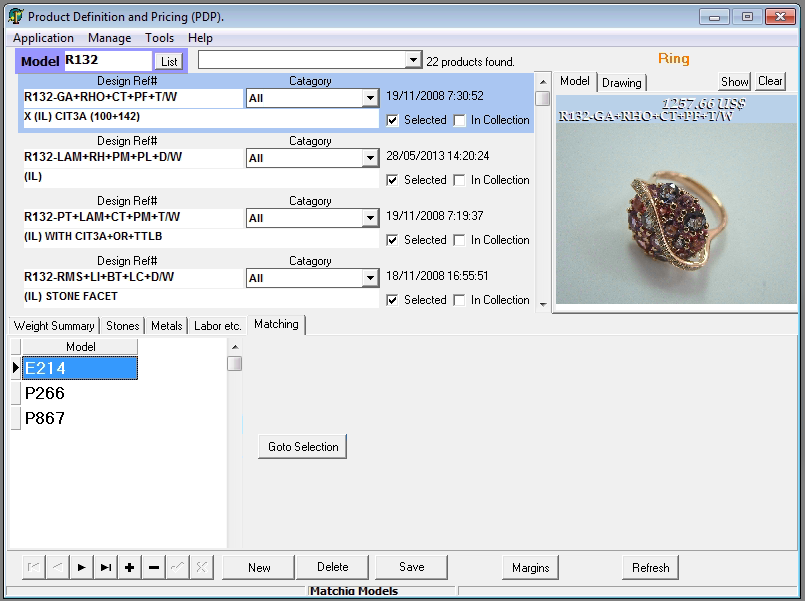
\includegraphics[width=0.4\textwidth]{./images/pdp_model_matching.png}
  \caption{Matching Items}
\end{figure}
Suggests complementary items (e.g.\ earrings and pendant matching a ring).

\subsection*{Manage Stones And Diamonds}
On the toolbar, under \texttt{Manage} → \texttt{Stones And Diamonds}, you have:

\subsubsection*{Types, Shapes etc.}
\paragraph{Categories and Types}
\begin{figure}[H]
  \centering

  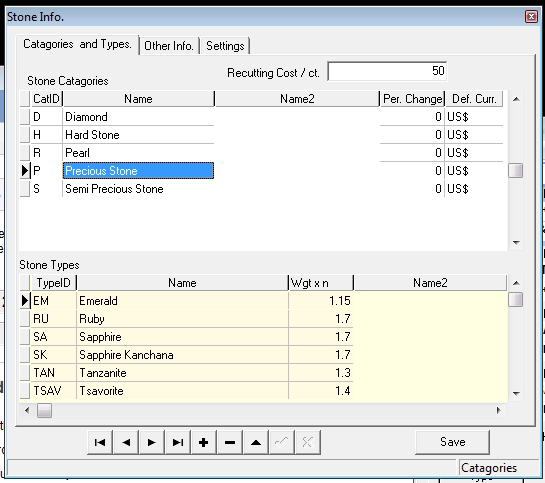
\includegraphics[width=0.4\textwidth]{./images/pdp_stonesinfos_categorysandtypes.png}
  \caption{Stone Categories \& Types}
\end{figure}
Table shows \texttt{TypeID}, \texttt{Name}, \texttt{Wgt x n} (density).

\paragraph{Other Info}
\begin{figure}[H]
  \centering

  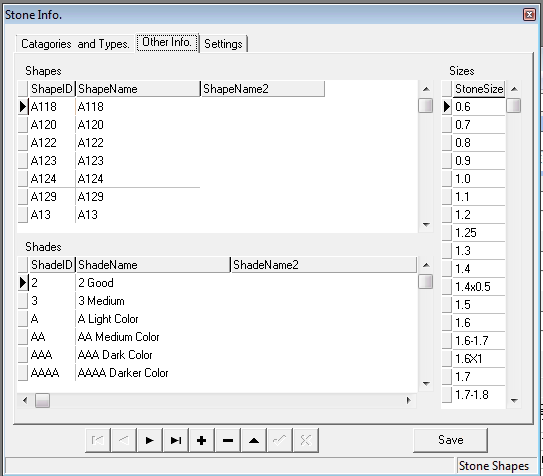
\includegraphics[width=0.4\textwidth]{./images/pdp_stonesinfos_otherinfo.png}
  \caption{Stone Other Info}
\end{figure}
Manage shapes, shades, sizes.

\paragraph{Settings}
\begin{figure}[H]
  \centering

  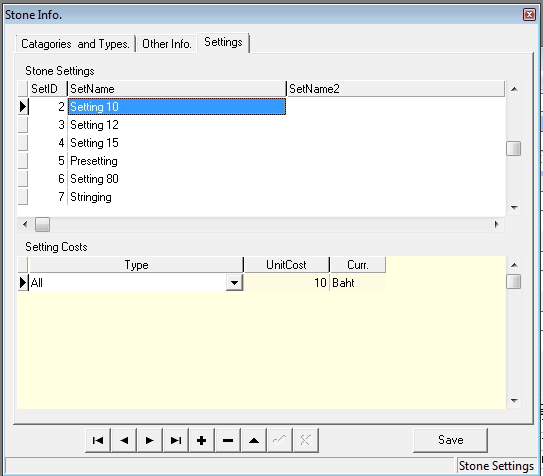
\includegraphics[width=0.4\textwidth]{./images/pdp_stonesinfos_settings.png}
  \caption{Stone Settings}
\end{figure}
Labor cost settings for different setting types.

\subsubsection*{Unit Costs}
\begin{figure}[H]
  \centering

  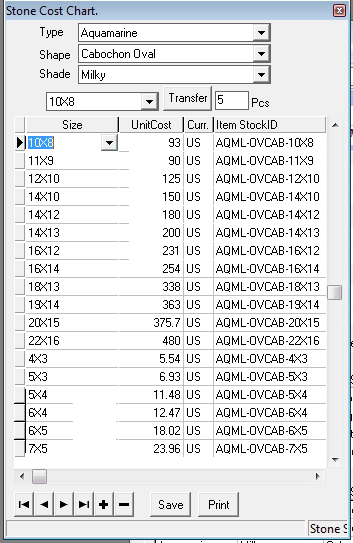
\includegraphics[width=0.4\textwidth]{./images/pdp_stonecostchart.png}
  \caption{Stone Cost Chart}
\end{figure}
Manage prices per stone; print PDF with \texttt{Print}.

\begin{figure}[H]
  \centering

  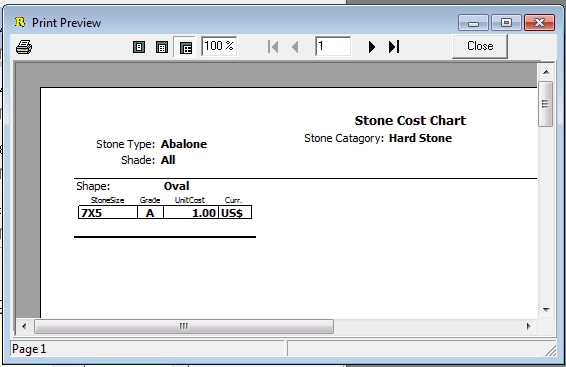
\includegraphics[width=0.4\textwidth]{./images/pdp_stonecostchar_print.png}
  \caption{Print View}
\end{figure}

\subsubsection*{Unit Weights}
\begin{figure}[H]
  \centering

  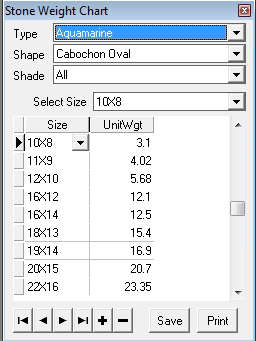
\includegraphics[width=0.4\textwidth]{./images/pdp_stoneweightchart.png}
  \caption{Stone Weight Chart}
\end{figure}

\subsection*{Manage Metals}
\begin{figure}[H]
  \centering

  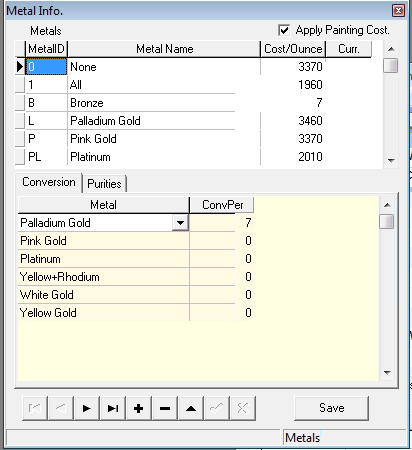
\includegraphics[width=0.4\textwidth]{./images/pdp_metalinfo.png}
  \caption{Metal Info}
\end{figure}
Conversion and purity tables:

\begin{figure}[H]
  \centering

  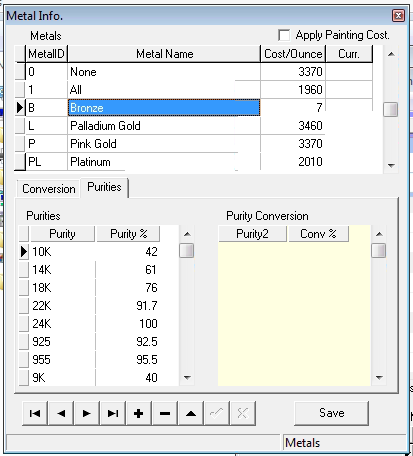
\includegraphics[width=0.4\textwidth]{./images/pdp_metalinfo_purities.png}
  \caption{Purities}
\end{figure}

\subsection*{Manage Parts}
\begin{figure}[H]
  \centering

  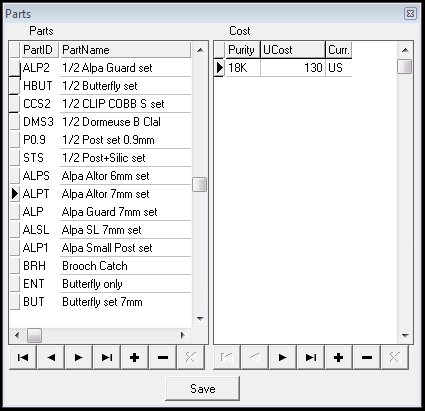
\includegraphics[width=0.4\textwidth]{./images/pdp_parts.png}
  \caption{Parts Database}
\end{figure}

\subsection*{Manage Margins}
By default: \emph{Misc} sub-view.

\begin{figure}[H]
  \centering

  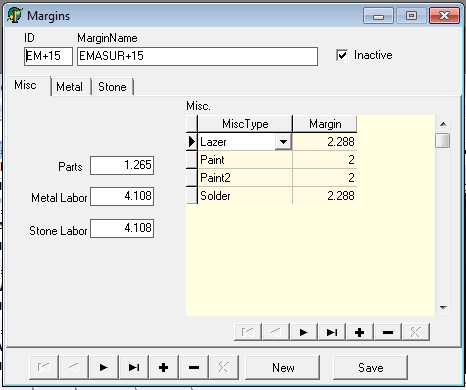
\includegraphics[width=0.4\textwidth]{./images/pdp_margins_misc.png}
  \caption{Misc Margins}
\end{figure}

Metal sub-view:

\begin{figure}[H]
  \centering

  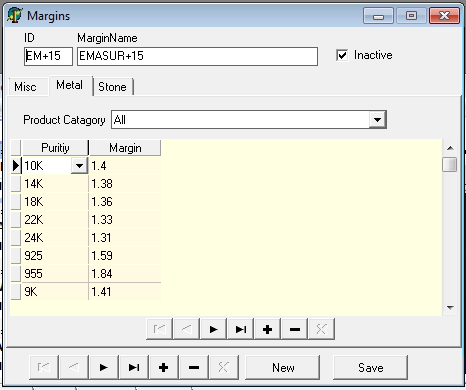
\includegraphics[width=0.4\textwidth]{./images/pdp_margins_metal.png}
  \caption{Metal Margins}
\end{figure}

Stone conditional:

\begin{figure}[H]
  \centering

  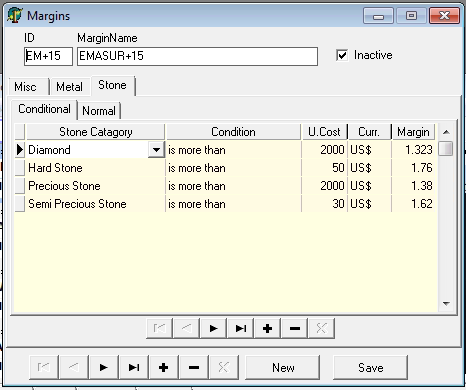
\includegraphics[width=0.4\textwidth]{./images/pdp_margins_stone_conditionnal.png}
  \caption{Stone Conditional Margins}
\end{figure}

Stone normal:

\begin{figure}[H]
  \centering

  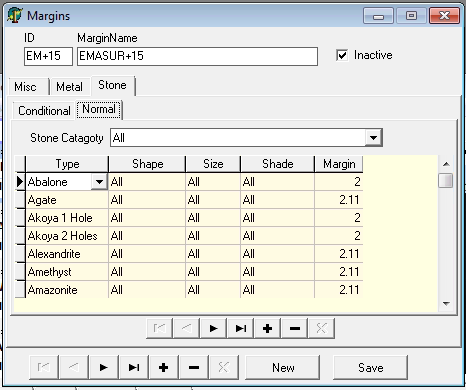
\includegraphics[width=0.4\textwidth]{./images/pdp_margins_stone_normal.png}
  \caption{Stone Normal Margins}
\end{figure}

\subsection*{Manage Ornament Categories}
\begin{figure}[H]
  \centering

  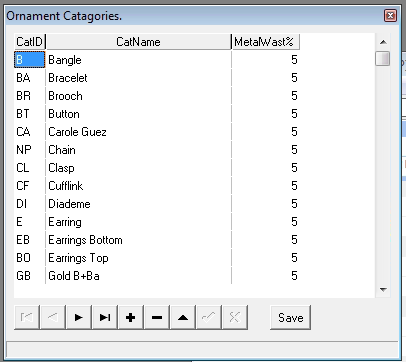
\includegraphics[width=0.4\textwidth]{./images/pdp_ornementcategories.png}
  \caption{Ornament Categories}
\end{figure}

\subsection*{Manage Currencies}
\begin{figure}[H]
  \centering

  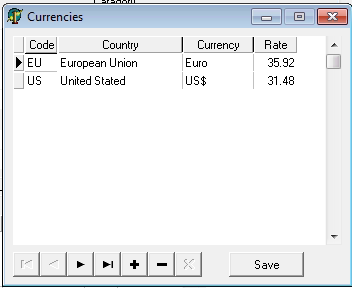
\includegraphics[width=0.4\textwidth]{./images/pdp_currencies.png}
  \caption{Currencies}
\end{figure}

\subsection*{Tools}
Toolbar → \texttt{Tools}:
\begin{description}[leftmargin=*]
  \item[Options] \begin{figure}[H]
  \centering

      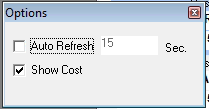
\includegraphics[width=0.4\textwidth]{./images/pdp_tools_option.png}
      \caption{Options}
    \end{figure}
  \item[Reports] \begin{figure}[H]
  \centering

      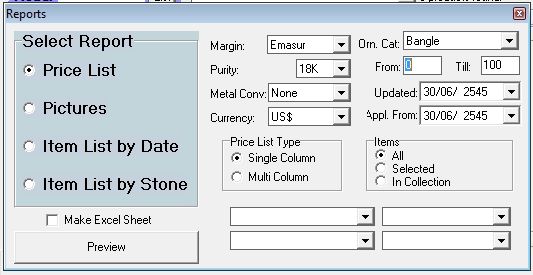
\includegraphics[width=0.4\textwidth]{./images/pdp_tools_reports.png}
      \caption{Reports}
    \end{figure}
  \item[Check Data] \begin{figure}[H]
  \centering

      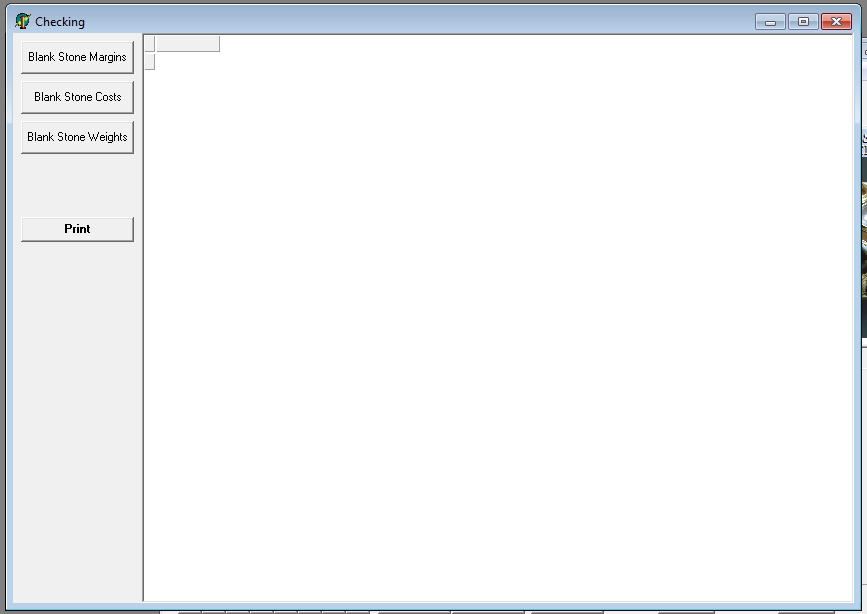
\includegraphics[width=0.4\textwidth]{./images/pdp_tools_checkdata.png}
      \caption{Check Data}
    \end{figure}
\end{description}

\subsection*{Processes}

\subsubsection*{Create a new \textbf{Model}}
\begin{enumerate}[leftmargin=*]
  \item From main page, click \texttt{List} next to \texttt{Model XXXX}.
  \item Select type and last model \texttt{AAXXXB}.
  \item Click \texttt{Select}, increment the model number (\texttt{AA(XXX+1)B}), press \texttt{Enter}.
  \item Click \texttt{Save}, then \texttt{New}.
  \item Enter new design reference \texttt{AAYYYB-CS+S1+\dots/W}, click \texttt{Make Blank}.
  \item Fill Stones, Metals, Labor tables, saving after each.
\end{enumerate}

\subsubsection*{Create a new \textbf{Reference} (Product)}
\begin{enumerate}[leftmargin=*]
  \item Search model \texttt{AAXXXB} and press \texttt{Enter}.
  \item Click \texttt{New}, choose design, enter new reference, click \texttt{Copy}.
  \item Fill Stones and adjust Labor tables if needed, saving after each.
\end{enumerate}

\subsubsection*{Add Type of Stone}
\begin{enumerate}[leftmargin=*]
  \item \texttt{Manage} → \texttt{Stones And Diamonds} → \texttt{Types, Shape etc.}
  \item Select Category, click \texttt{+}, fill \texttt{TypeID}, \texttt{Name}, \texttt{Wgt x n}, click \texttt{Save}.
  \item Handle errors if not unique.
\end{enumerate}

\subsubsection*{Add Specific Stone}
\begin{enumerate}[leftmargin=*]
  \item \texttt{Manage} → \texttt{Unit Costs}, select attributes, click \texttt{+}, fill \texttt{Size}, \texttt{UnitCost}, save.
  \item \texttt{Manage} → \texttt{Unit Weights}, select attributes, click \texttt{+}, fill \texttt{Size}, \texttt{UnitWgt}, save.
\end{enumerate}
